\section{\texorpdfstring{Rekurzivní funkce}{Rekurzivní funkce}}

% =====================================================================================================================
	\begin{frame}
    \frametitle{Rekurze}
		
		\begin{itemize}
			\item Proces při kterém se objekt nebo funkce odkazuje sama na sebe,
			\item funkce odkazující na sama sebe je \textbf{rekurzivní funkcí},
			\item sama rekurze je využívána v případech, kdy problém lze dělit na menší celky se stejným algoritmem řešení.
		\end{itemize}
		
		\vspace{4mm}
		\textbf{Příklad:} Výpočet Fibonacciho posloupnosti
		\begin{align*}
			F_n =& F_{n-1} + F_{n-2} \\
			F_0 =& 0 \\
			F_1 =& 1
		\end{align*}
		
		\begin{itemize}
			\item na procesu výpočtu ukážeme předání parametru, založení lokální proměnné a vrácení hodnoty.
		\end{itemize}
	\end{frame}
	
% =====================================================================================================================
	\begin{frame}
    \frametitle{Příklad programu Fibonacci v jazyce C}
		\small
		\begin{center}
			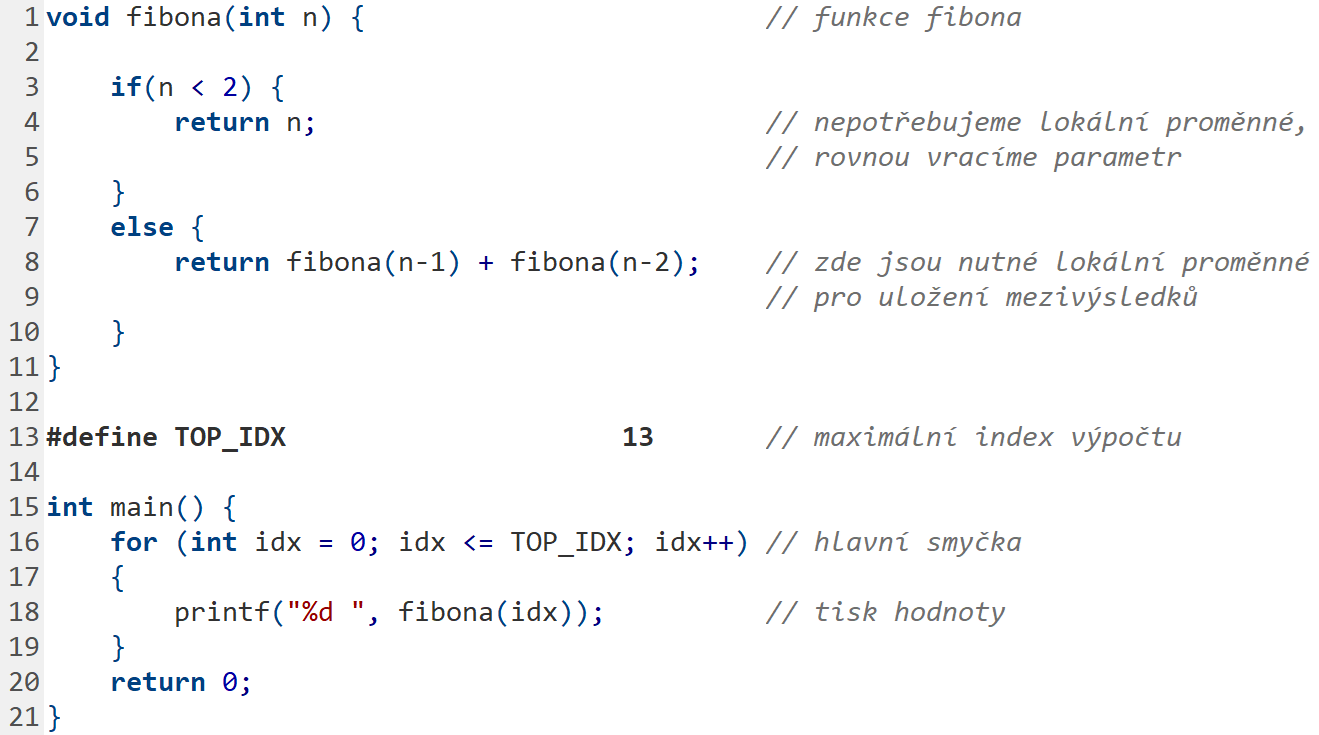
\includegraphics[width=0.80\textwidth]{fig/prg_fib_c.png}
		\end{center}
		
		\begin{itemize}
			\item V asembleru zachováme význam proměnných a konstant,
			\item výpis \textbf{printf} nahradíme zobrazením na LED přípravku.
		\end{itemize}
		
	\end{frame}
	
% =====================================================================================================================
	\begin{frame}
    \frametitle{Program Fibonacci - Definice symbolických konstant}
		\small
		\begin{center}
			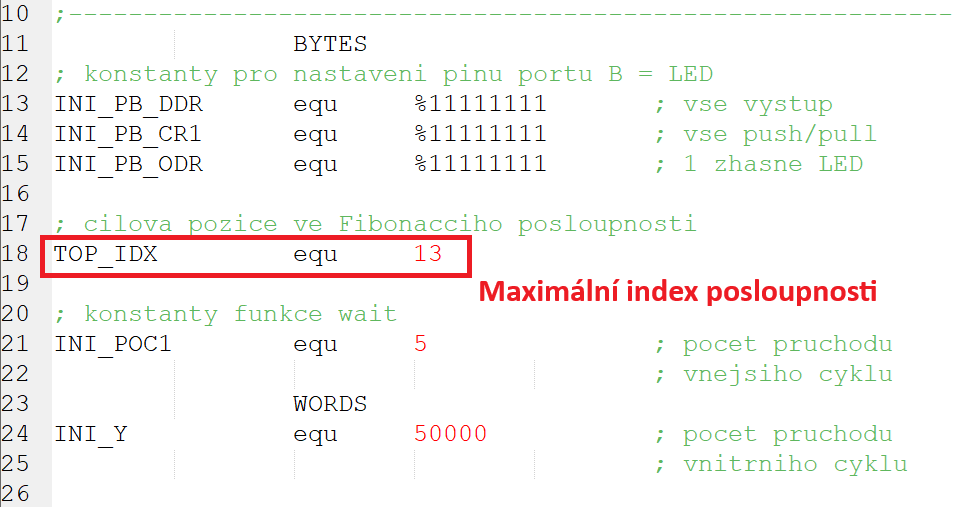
\includegraphics[width=0.90\textwidth]{fig/prg_fib_definice.png}
		\end{center}
		
		
		\begin{itemize}
			\item Definujeme \textbf{TOP\_IDX}.
		\end{itemize}
		
	\end{frame}
	
% =====================================================================================================================
	\begin{frame}
    \frametitle{Program Fibonacci - Inicializace}
		\small
		\begin{center}
			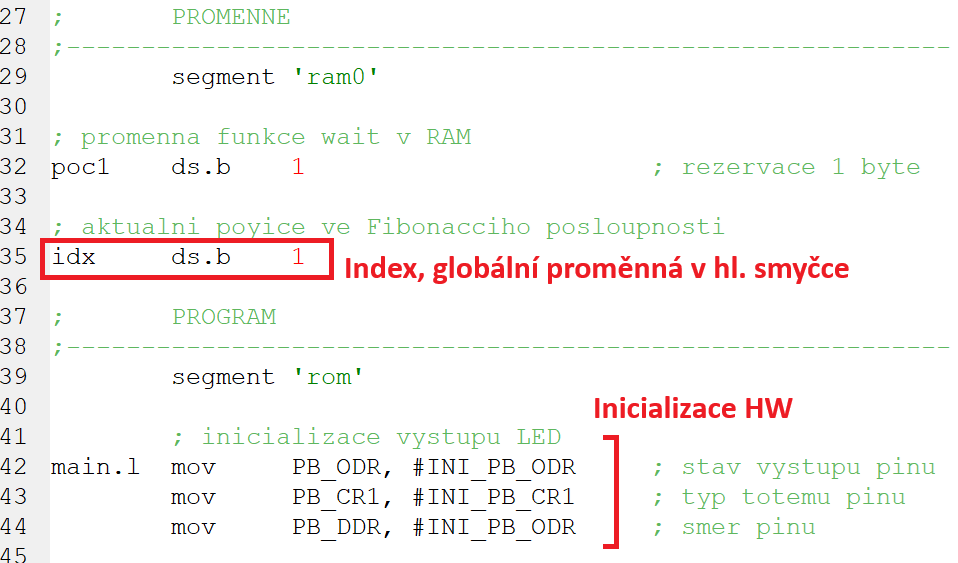
\includegraphics[width=0.90\textwidth]{fig/prg_fib_varini.png}
		\end{center}
		
	\end{frame}
	
% =====================================================================================================================
	\begin{frame}
    \frametitle{Program Fibonacci - Hlavní smyčka}
		\small
		\begin{center}
			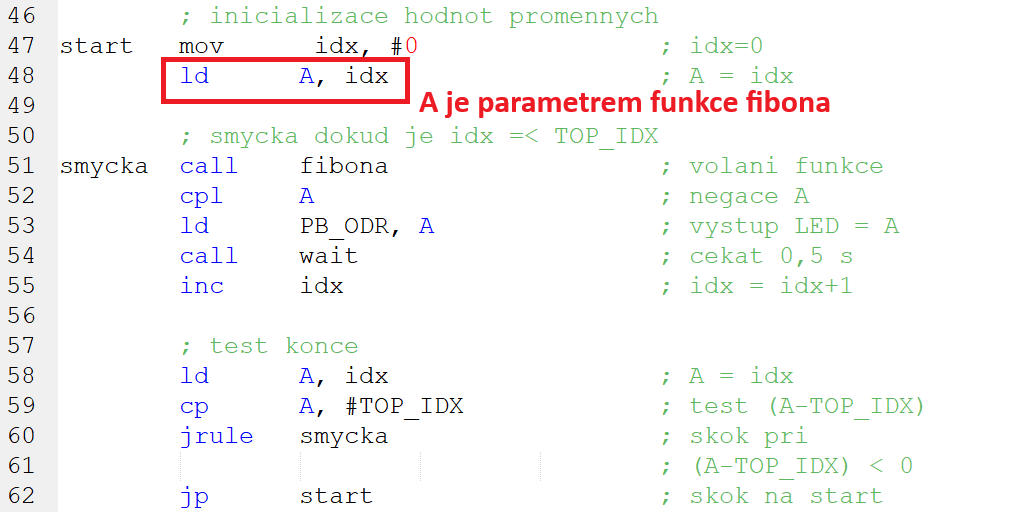
\includegraphics[width=0.90\textwidth]{fig/prg_fib_smycka.png}
		\end{center}
		
		\begin{itemize}
			\item Provedeme \textbf{TOP\_IDX+1} průchodů a výsledky funkce \textbf{fibona} zobrazíme na LED.
		\end{itemize}
	\end{frame}

% =====================================================================================================================
	\begin{frame}
    \frametitle{Program Fibonacci - Funkce \textbf{fibona}}
		\small
		\begin{center}
			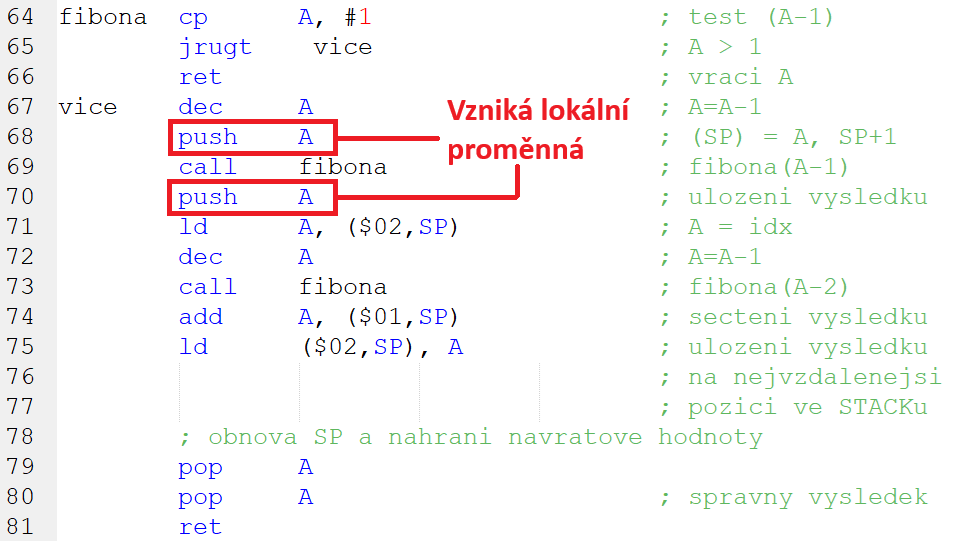
\includegraphics[width=0.90\textwidth]{fig/prg_fib_funkce.png}
		\end{center}
		
	\end{frame}
	
% =====================================================================================================================
	\begin{frame}
    \frametitle{Doporučení}
		
		\small
		\begin{itemize}
			\item Program krokujte v simulátoru nebo v přípravku,
			\item zobrazte si paměť \textbf{RAM} na pozici \textbf{0x07FF} (oblast zásobníku - \textbf{STACK}),
			\item pozorujte jak roste využití zásobníku,
			\item v extrémním případě vysokého indexu může dojít k vyčerpání celého vyhrazeného prostoru a tím k přetečení zásobníku \\ 		$\Longrightarrow$ \textbf{STACK OVERFLOW}.
		\end{itemize}
		
		\begin{center}
			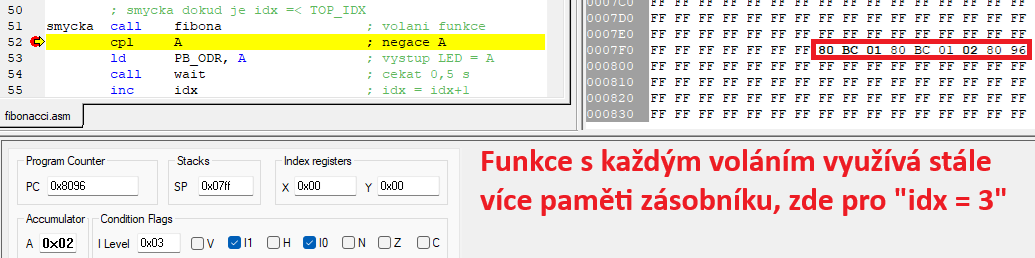
\includegraphics[width=1.00\textwidth]{fig/stack_fill.png}
		\end{center}
		
	\end{frame}